\documentclass[a4,german]{article}

\usepackage[german]{babel} % für deutsche Silbentrennung und generierte Texte
\usepackage[T1]{fontenc}    % für deutsche Umlaute etc. in der Ausgabe
\usepackage[utf8]{inputenc} % für deutsche Umlaute.
\usepackage{graphicx}       % um Bilder einzubinden
\usepackage{hyperref}       % um URLs korrekt einzubinden und Hyperlinks im Dokument zu ermöglichen
\usepackage{subcaption}


\begin{document}

\title{Klassifizierung von Früchten}
\author{Henry Apostle, Sibel Gül, Robert Johanson und Darwin Willers}

\maketitle % setzt automatisch den angegebenen Autor und Titel, sowie das ehutige Datum als Überschirft (weitere Angaben möglich)


\begin{abstract}

\end{abstract}

\section{Einleitung}

\section{Daten}
Der verwendete Datensatz stammt von zenodo.org. Ursprünglich bestand er aus 44.406 Bildern verteilt auf 15 Klassen. Da wir eine zusätzliche Unterscheidung zwischen grünen und roten Äpfeln machten, kamen wir auf 16 Klassen. Pro Klasse haben wir anschließend 1.000 Bilder zufällig ausgewählt und somit den Datensatz auf eine Größe von 16.000 Bildern reduziert. Die 16 Klassen sind: grüner Apfel, roter Apfel, Banane, Sternfrucht, Guave, Kiwi, Mango, Zuckermelone, Orange, Pfirsich, (Nashi-)Birne, Kaki, Drachenfrucht, Pflaume, Granatapfel und Tomate. Abbildung 1 zeigt je ein exemplarisches Bild aus jeder Klasse. Alle Bilder sind 320x258 Pixel groß. Weiterhin ist allen Bildern gemeinsam, dass das Obst auf einem grau/silbernem Blech abfotografiert wurde. Unterschiede gibt es in der Belichtung, der Anzahl und der Anordnung der Früchte auf dem Blech. Des Weiteren wurden einige Bilder im Nachhinein gedreht und verzerrt [genauer], während auf anderen noch eine Hand zu sehen ist (siehe Abbildung 2). Auffallend am Datensatz ist, dass es sich bei mehreren Klassen um rundes grünes Obst handelt, nämlich bei grüner Apfel, Guave, Zuckermelone, Birne und oftmals auch Granatapfel. Bei der Zuckermelone gibt es manche Bilder, die wir als grünen Apfel klassifiziert hätten (z.B siehe Abbildung 3). Bei der Birne handelt es sich um die Nashi Birne, die eben nicht der gewöhnlichen Form einer Birne entspricht und die man optisch auch leicht mit grünen Äpfeln verwechseln kann. Des Weiteren sind die Granatäpfel auf den Bildern oft sehr unreif und somit eher grün. 

\begin{figure}[b] % jedes Bild kommt in seine eigene Figure-Umgebung
\begin{center} % zentrieren des Bild
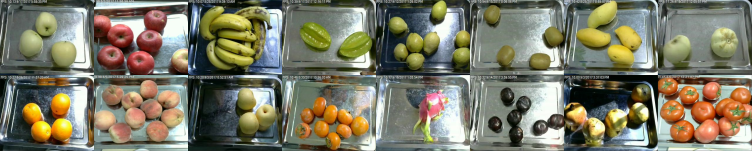
\includegraphics[width=1\linewidth]{16fruits.png}
\caption{Die 16 verschiedenen Früchte, die klassifiziert werden. Von oben links nach unten rechts sind das: grüner Apfel, roter Apfel, Banane, Sternfrucht, Guave, Kiwi, Mango, Zuckermelone, Orange, Pfirsich, Birne, Kaki, Drachenfrucht, Pflaume, Granatapfel und Tomate.
\label{fig:16fruits} % Label, unter dem das Bild mit \ref referenziert werden kann
}
\end{center}
\end{figure}

\begin{figure}[b] % jedes Bild kommt in seine eigene Figure-Umgebung
\begin{subfigure}[c]{0.245\textwidth}
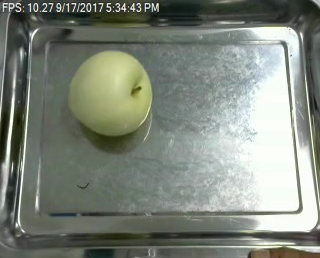
\includegraphics[width=1\textwidth]{Apple_Green_44.png} 
\subcaption{}
\end{subfigure}
\begin{subfigure}[c]{0.245\textwidth}
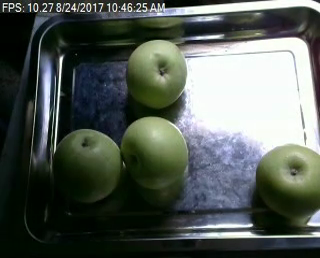
\includegraphics[width=1\textwidth]{Apple_Green_50.png}
\subcaption{}
\end{subfigure}
\begin{subfigure}[c]{0.245\textwidth}
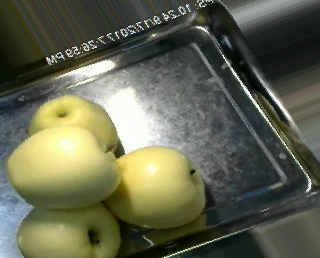
\includegraphics[width=1\textwidth]{Apple_Green_10.png}
\subcaption{}
\end{subfigure}
\begin{subfigure}[c]{0.245\textwidth}
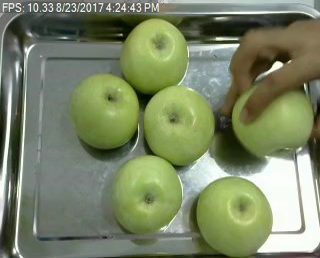
\includegraphics[width=1\textwidth]{Apple_Green_0.png}
\subcaption{}
\end{subfigure}
\caption{Auf diesen vier Bildern sind Unterschiede zu erkennen, die man innerhalb einer Klasse begegnen kann. Alle Bilder zeigen grüne Äpfel. Bei (a) und (b) erkennt man Unterschiede in der Anzahl der Äpfel und in der Belichtung, (c) wurde gedreht und verzerrt und auf (d) ist eine Hand zu sehen.}
\end{figure}

\begin{figure}[b] % jedes Bild kommt in seine eigene Figure-Umgebung
\begin{subfigure}[c]{0.19\textwidth}
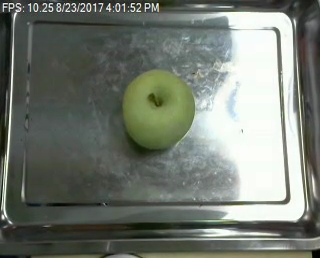
\includegraphics[width=1\textwidth]{Apple_Green_60.png} 
\subcaption{}
\end{subfigure}
\begin{subfigure}[c]{0.19\textwidth}
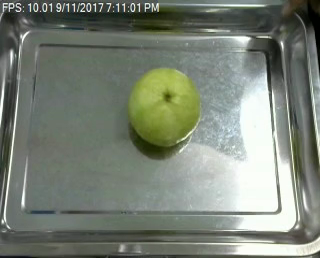
\includegraphics[width=1\textwidth]{Guava_21.png}
\subcaption{}
\end{subfigure}
\begin{subfigure}[c]{0.19\textwidth}
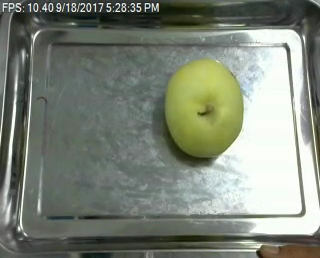
\includegraphics[width=1\textwidth]{Muskmelon_11.png}
\subcaption{}
\end{subfigure}
\begin{subfigure}[c]{0.19\textwidth}
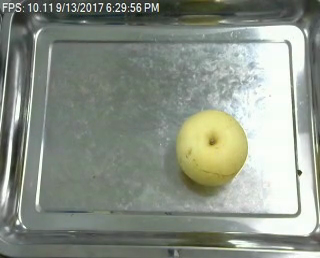
\includegraphics[width=1\textwidth]{Pear_8.png}
\subcaption{}
\end{subfigure}
\begin{subfigure}[c]{0.19\textwidth}
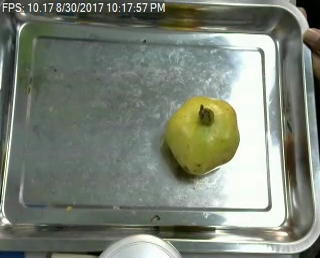
\includegraphics[width=1\textwidth]{Pomegranate_534.png}
\subcaption{}
\end{subfigure}
\caption{Hier sind fünf grüne runde Früchte zu sehen, welche eine Gefahr für die Klassifikation sein könnten: (a) grüner Apfel, (b) Guave, (c) Zuckermelone, (d) Birne und (e) Granatapfel.}
\end{figure}

\section{Methodik}

Als wesentliches Merkmal zur Unterscheidung der Früchte dient uns die Farbe. Form haben wir an dieser Stelle vernachlässigt, da auf den Bildern das Obst in unterschiedlicher Anzahl und Anordnung gegeben ist. Manchmal liegen die Früchte nebeneinander, manchmal sind sie sogar gestapelt. Somit müsste man erst ein Programm schreiben, dass eine einzelne Frucht lokalisiert, um dann anschließend ihre Form auszuwerten. Dies fanden wir zu kompliziert, besonders da das alleinige Betrachten der Farbe schon für sehr gute Ergebnisse ausreicht.\\
Unser Programm durchläuft mehrere Schritte: Zuerst wird das Obst vom Hintergrund mittels Binarisierung getrennt, anschließend wird das 'ausgeschnittene' Bild mittels 3D-Histogramm in farbliche Komponenten zerlegt und zuletzt wird mittels Nearest-Neighbour-Klassifikator bestimmt zu welcher Obstsorte das Bild gehört. Im Folgenden gehen wir auf die einzelnen Schritte genauer ein:\\

\subsection{Das Ausschneiden}
Um das Obst von dem Blech zu unterscheiden, haben wir beobachtet, dass die Farben der Früchte deutlich saturierter sind, als das Grau/Silber des Blechs. Deshalb transformiert unser Programm das Bild zuallererst in den HSV-Raum, wo wir dann nur den S-Kanal (die Saturation) betrachten. Darauf wenden wir anschließend das Otsu-Verfahren an. [Otsu macht diesdas].
[siehe Abbildung 4]

\begin{figure}[b] % jedes Bild kommt in seine eigene Figure-Umgebung
\begin{subfigure}[c]{0.245\textwidth}
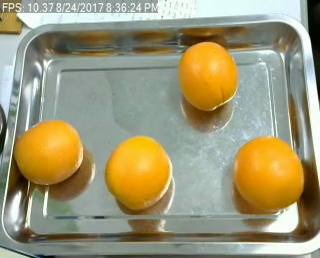
\includegraphics[width=1\textwidth]{TestBild.png} 
\subcaption{Input}
\end{subfigure}
\begin{subfigure}[c]{0.245\textwidth}
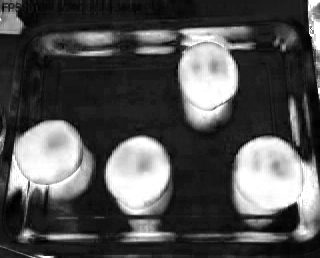
\includegraphics[width=1\textwidth]{TestBildS.png}
\subcaption{S-Kanal}
\end{subfigure}
\begin{subfigure}[c]{0.245\textwidth}
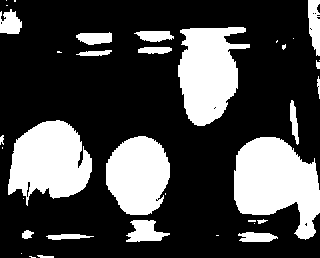
\includegraphics[width=1\textwidth]{TestMask.png}
\subcaption{Binarisiertes Bild}
\end{subfigure}
\begin{subfigure}[c]{0.245\textwidth}
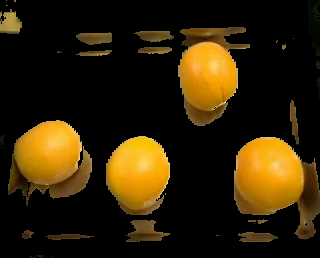
\includegraphics[width=1\textwidth]{TestAusgeschnitten.png}
\subcaption{Ausgeschnitten}
\end{subfigure}
\caption{Auf diesen vier Bildern ist der Prozess des Ausschneidens verdeutlicht. Bild (a) zeigt ein Beispielbild. Dieses wird in den HSV-Raum transformiert und Bild (b) zeigt den entsprechenden Saturation Kanal. Darauf wird das Otsu-Verfahren angewandt und es entsteht das binarisierte Bild (c). Aus (a) und (c) lässt sich das ausgeschnittene Bild (d) ableiten.}
\end{figure}

\subsection{3D-Histogramm}
[So funktioniert ein 3D-Histogramm]\\

[Das Normieren erwähnen]

\subsection{Nearest-Neighbor Klassifikator}
[So funktioniert der NN Klassifikator]

\section{Experimente}
Pro Klasse hatten wir 800 Trainings- und 200 Testbilder. Insgesamt also 12.800 Trainings- und 3.200 Testbilder. Unser Programm hat die 3.200 Testbilder zu 96,34\% korrekt zugeordnet. Im Folgenden gehen wir die einzelnen Komponenten unseres Systems durch und schauen, wie sich die Trefferquote ändert, wenn wir sie austauschen:\\
Wenn wir die Bilder nicht ausschneiden, sondern direkt in 3D-Histogramme verwandeln und mit dem Nearest-Neighbour Klassifikator klassifizieren erhalten wir immer noch eine Trefferquote von 93,09\%. Tatsächlich selbst wenn wir den 3D-Histogramm durch den kanalweisen Mittelwert ersetzen, erhalten wir immer noch eine Trefferquote von 51,28\% auf den nicht ausgeschnittenen Bildern. Dies erklären wir uns dadurch, dass wir einerseits eine sehr hohe Menge an Trainingsbildern haben und andererseits die Bilder im Großen und Ganzen doch ziemlich ähnlich sind. Wenn wir aber den Mittelwert aber auf den ausgeschnittenen Bildern anwenden liegt die Trefferquote sogar bei 77,5\%. Dies zeigt, dass es durchaus etwas bringt, die Bilder auszuschneiden.\\

[Andere Deskriptoren betrachten]\\

[Andere Klassifikatoren (k-Nearest Neighbour) betrachten]\\

[Man kann dann auch Bilder zeigen, die unser Programm falsch erkennt. Die sind im Ergebnisse.pdf aufgelistet.]


\section{Schluss}


% Literaturverzeichnis mit Hilfe der "thebibliography" Umgebung:

\begin{thebibliography}{99}
	
% Beispiel für ein Buch
%\bibitem {kopka96} H. Kopka. \textit{LaTeX - eine Einführung}. Addison-Wesley, 1996.
% Beispiel für einen Zeitschriftenartikel
%\bibitem {viola_jones04} P. Viola and M. J. Jones. Robust real-time face detection. \textit{International Journal of Computer Vision} (IJCV), 57(2):137-154, May 2004.
% Beispiel für eine Doktorarbeit (Bachelor-, Masterarbeiten analog)
%\bibitem {frintrop_phd05} S. Frintrop. \textit{VOCUS: A Visual Attention System for Object Detection and Goal-directed Search.} PhD thesis, Rheinische Friedrich-Wilhelms Universität Bonn, Germany, July 2005. 
https://zenodo.org/record/1310165
\end{thebibliography}



\end{document}
